\documentclass{standalone}
\usepackage{tikz}
\usepackage{ctex,siunitx,bm}
\setCJKmainfont{Noto Serif CJK SC}
\usepackage{tkz-euclide}
\usepackage{amsmath}
\usetikzlibrary{patterns, calc}
\usetikzlibrary {decorations.pathmorphing, decorations.pathreplacing, decorations.shapes,}
\begin{document}
\small
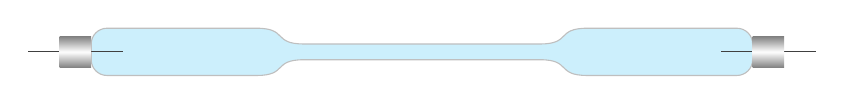
\begin{tikzpicture}[>=latex,yscale=1.0]
  \fill[cyan!20!white,draw=lightgray](4.2,0.1)arc(0:90:0.2)--(2.1,0.3)..controls(1.7,0.3)and(1.9,0.1)..(1.5,0.1)--(-1.5,0.1)..controls(-1.9,0.1)and(-1.7,0.3)..(-2.1,0.3)--(-4.0,0.3)arc(90:180:0.2)--(-4.2,-0.1)arc(180:270:0.2)--(-2.1,-0.3)..controls(-1.7,-0.3)and(-1.9,-0.1)..(-1.5,-0.1)--(1.5,-0.1)..controls(1.9,-0.1)and(1.7,-0.3)..(2.1,-0.3)--(4.0,-0.3)arc(270:360:0.2)--cycle;
  \draw[thin,darkgray](-5,0)--++(1.2,0)(5,0)--++(-1.2,0);
  \fill[top color=gray,bottom color=gray, middle color=white]
  (-4.2,0.2)rectangle(-4.6,-0.2);
  \fill[top color=gray,bottom color=gray, middle color=white]
  (4.2,0.2)rectangle(4.6,-0.2);
\end{tikzpicture}
\end{document}